\documentclass{article}
\usepackage[utf8]{inputenc}
\usepackage{amsmath}
\usepackage{amssymb}
\usepackage{amsfonts}
\usepackage{amssymb}
\usepackage{minted}
\usepackage{graphicx}
\usepackage{algorithm}
\usepackage{algpseudocode}
\graphicspath{ {img/} }
\usepackage{titlesec}
\usepackage[a4paper,margin=1in,footskip=0.25in]{geometry}
\usepackage{fancyhdr}
\pagestyle{fancy}
%basic page layout

%draw finite state machine
\usepackage{tikz}
\usetikzlibrary{arrows,automata}
\newcommand{\hwnumber}{4}
\newcommand{\Lcvy}{\mathcal{L}}
%header and footer settings
\lhead{Algorithms and Data Structure \hwnumber}
\chead{Yiping Deng}
\rhead{\today}

\titlelabel{\thetitle\enspace}

\begin{document}
\title{Algorithms and Data Structure \hwnumber}
\author{Yiping Deng}
\maketitle
\thispagestyle{fancy}
\section*{Problem 1}
\subsection*{a)}
The algorithm for bubble sort is shown in \ref{bubblesort}
\begin{algorithm}
    \caption{Bubble Sort}
    \label{bubblesort}
    \begin{algorithmic}[1]
        \Procedure{BubbleSort}{$A$}
        \Comment{Input a array $A$}
        \State $swapped \gets true$
        \Comment{Make sure it will execute at least once}
        \While {swapped}
        \Comment{Keep executing until it is sorted}
        \State $swapped \gets false$
        \For {$i$ from 1 to A.size - 1}
        \If{$A[i] \geq A[i + 1]$}
        \State $swapped \gets true$
        \State $swap(A[i], A[i + 1])$
        \Comment{Swap two misplaced elements in the array}
        \EndIf
        \EndFor
        \EndWhile
        \EndProcedure
    \end{algorithmic}
\end{algorithm}
\subsection*{b)}
\textbf{Best Case:} If the array is already sorted, the if condition is never satisfied, and the loop
is executed once, which will give us $O(n)$ comparisions, and it is also its running time. \\
\textbf{Worst Case:} If the array is inversely sorted, the last element in the original array $A$
will be swapped to the front(its correct position) in $n - 1$ loops, with one extra loop of termination. Still, the number of comparision
will be $O((n - 1) \cdot n) = O(n^2)$ \\
\textbf{Average Case:} On uniform distributed array $A$, bubble sort's number of loops are bounded
below by $n / 2$, and bounded above by $n$, so it is $O(n)$ loop, with each loop takes $O(n)$. It implies
a running time of $O(n) \cdot O(n) = O(n^2)$
\subsection*{c)}
\begin{itemize}
    \item Insertion Sort: Stable sort. If two element is in sorted order, it will not be swapped.
    \item Merge Sort: Stable sort. If the merge operation is properly implemented, it will preserve
        the relative order of the object. In the split operation, order is preserved completely.
    \item Heap Sort: Unstable sort. The sorted array is derived from continuously popping elements from
        the heap. However, the heapify operation will break the relative ordering.
    \item Bubble Sort: Stable sort. You will not swap any element in a sorted order, and it keeps the
        relative order in the list.
\end{itemize}
\subsection*{d)}
\begin{itemize}
    \item Insertion Sort: Adaptive. The best case is linear while the average case is quadratic.
    \item Merge Sort: Not adaptive. The number of merge operation does not change.
    \item Heap Sort: Not adaptive. Number of heapify call does not change.
    \item Bubble Sort: Adaptive. The best case is linear while the average case is quadratic.
\end{itemize}
\section*{Problem 2}
\subsection*{a)}
Code is here for HeapSort.scala
\inputminted{Scala}{HeapSort/src/main/scala/HeapSort.scala}
\subsection*{b)}
The variant code is here
\inputminted{Scala}{HeapSort/src/main/scala/HeapSortVariant.scala}
Also the test case for both algorithm, proving its correctness.
\inputminted{Scala}{HeapSort/src/test/scala/HeapSortTest.scala}
\subsection*{c)}
The original implementation is actually faster.
Consider the floating process, the original process take $O(lg(n))$ times to put in
the right position. While in our case, the floating means more swap operation on the entire array,
and in most of the case, the root and its two direct child
is not in the right position. Thus, it turns out it will
be slower. 
Because the Prof. explicit mentioned a different way of floating,
I do not use heapify function to float it down and fix the head.
If you use the code above to generate the data, and draw the graph using python code,
you can see it clearly. The green one is much slower.
\inputminted{Python}{draw.py}
Let's present the graph here. \\
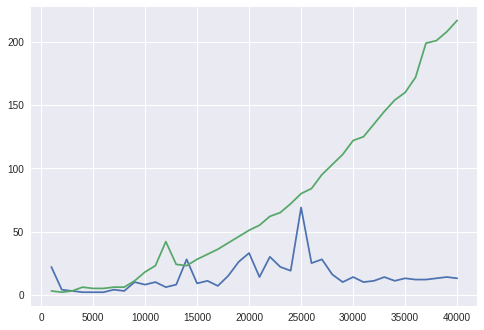
\includegraphics{draw.png}
\end{document}
